\documentclass{article}
\usepackage{amsmath, amssymb, color, xcolor, amsthm}
\usepackage{graphicx, wrapfig, float, caption, dsfont, bbm, xfrac}
\usepackage{fullpage}
\usepackage[backref=page, hidelinks, colorlinks=true, citecolor=blue!60!black!100]{hyperref}
\usepackage{tikz}
\usetikzlibrary{arrows.meta, shapes}
\usepackage{caption, subcaption}
\usepackage{natbib} % gives us \citet: Author (year) and \citep: (Author; year)
\usepackage{authblk}
\usepackage{multicol}
\usepackage[bottom]{footmisc}

% for comments in margins or not
\newif\ifmargincomments
\margincommentsfalse
% \margincommentstrue
\ifmargincomments
    \usepackage{todonotes}
    \usepackage[left=1cm,right=6.5cm,top=3cm,bottom=3cm,nohead,nofoot,marginparwidth=6cm]{geometry}
    \newcommand{\plr}[1]{\todo[color=blue!25]{#1}}
    \newcommand{\js}[1]{\todo[color=green!25]{#1}}
    % inline comment version
    \newcommand{\plri}[1]{{\color{blue}\it #1}}
\else
    \newcommand{\plr}[1]{{\color{blue}\it #1}}
    \newcommand{\js}[1]{{\color{green}\it #1}}
    \newcommand{\plri}[1]{\plr{#1}}
\fi

\newif\ifsubmission
\submissiontrue
% \submissionfalse
\ifsubmission
    % % stuff for submission
    \usepackage{lineno}
    % allow line numbers around math environments
    % from https://tex.stackexchange.com/questions/43648/why-doesnt-lineno-number-a-paragraph-when-it-is-followed-by-an-align-equation
        \newcommand*\patchAmsMathEnvironmentForLineno[1]{%
          \expandafter\let\csname old#1\expandafter\endcsname\csname #1\endcsname
          \expandafter\let\csname oldend#1\expandafter\endcsname\csname end#1\endcsname
          \renewenvironment{#1}%
             {\linenomath\csname old#1\endcsname}%
             {\csname oldend#1\endcsname\endlinenomath}}% 
        \newcommand*\patchBothAmsMathEnvironmentsForLineno[1]{%
          \patchAmsMathEnvironmentForLineno{#1}%
          \patchAmsMathEnvironmentForLineno{#1*}}%
        \AtBeginDocument{%
        \patchBothAmsMathEnvironmentsForLineno{equation}%
        \patchBothAmsMathEnvironmentsForLineno{align}%
        \patchBothAmsMathEnvironmentsForLineno{flalign}%
        \patchBothAmsMathEnvironmentsForLineno{alignat}%
        \patchBothAmsMathEnvironmentsForLineno{gather}%
        \patchBothAmsMathEnvironmentsForLineno{multline}%
        }
\else
    % for the nice version
\fi

\newcommand{\jss}[1]{{\color{olive}\it #1}}
% \newcommand{\ddt}{\frac{d}{dt}}
\newcommand{\ddt}{\dot}
\newcommand{\ro}{{ro}}
\newcommand{\nro}{{\bar{r}o}}
\newcommand{\rno}{{r\bar{o}}}
\newcommand{\nrno}{{\bar{r}\bar{o}}}
\newcommand{\reachable}{\mathcal{R}}
\newcommand{\unobservable}{\bar{\mathcal{O}}}
\newcommand{\R}{\mathbb{R}}
\newcommand{\E}{\mathbb{E}}
\renewcommand{\P}{\mathbb{P}}
\newcommand{\var}{\mathop{\mbox{Var}}}
\newcommand{\cov}{\mathop{\mbox{Cov}}}
\newcommand{\tr}{\mathop{\mbox{tr}}} % trace
\newcommand{\pda}{\frac{\partial}{\partial A_{ij}}}
\newcommand{\ind}{\mathds{1}}
\newcommand{\grad}{\nabla}

\newcommand{\calH}{\mathcal{H}}
\newcommand{\diag}{\text{diag}}
\newcommand{\1}{\mathbbm{1}}

% the triple (A,B,C) as 'system' (not using)
\newcommand{\Sys}{\mathcal{S}}
% neutral set of all systems
\newcommand{\allS}{\mathcal{N}}

% fitness as a fn of distance
\newcommand{\fit}{\mathcal{F}}
% fitness as a fn of A
\newcommand{\fitx}{\mathcal{F}}
% optimal phenotype
\newcommand{\optph}{\Phi_0}
% distance in phenotype space
\newcommand{\dph}{d}
% incompatibility
\newcommand{\Incompat}{\mathcal{I}}

\DeclareMathOperator{\spn}{span}

\newtheorem{example}{Example}

% Responses to reviews
\usepackage{lineno, hyperref}
% \usepackage[hypertexnames=false]{hyperref}   % not working correctly
% \usepackage{latexml}

\linenumbers


%%%%%  PUT THIS IN HEADER OF FILE
% % Responses to reviews:
% \usepackage{lineno, hyperref}
% \usepackage[hypertexnames=false]{hyperref}   % not working correctly
% \usepackage{latexml}

\linenumbers


%%%%%  PUT THIS IN HEADER OF FILE
% % Responses to reviews:
% \usepackage{lineno, hyperref}
% \usepackage[hypertexnames=false]{hyperref}   % not working correctly
% \usepackage{latexml}

\linenumbers


%%%%%  PUT THIS IN HEADER OF FILE
% % Responses to reviews:
% \input{review-response-commands}
% % set this to show line numbers and include responses to reviews or not
% \newif\ifreviewresponses
% \reviewresponsestrue  % include them
% % \reviewresponsesfalse  % don't include them
% \newcommand{\responsefile}{pbio-reviews-19sept12-responses.tex}  % name of the review reponses file

% counters for reviewer points
%% instead do reviewer labels
% \newcounter{reviewer}
% \setcounter{reviewer}{0}
\newcommand{\thereviewer}{}
\newcounter{point}
\setcounter{point}{0}

% pass in to \reviewersection the label for this reviewer (i.e. \reviewersection{1} or \reviewersection{AE})
\newcommand{\reviewersection}[1]{\renewcommand{\thereviewer}{#1}
                  \setcounter{point}{0}
                  \section*{Reviewer \thereviewer:}}
% drawing from from http://tex.stackexchange.com/questions/2317/latex-style-or-macro-for-detailed-response-to-referee-report
%% arguments to \point are (name of the point, optional) and (content)
\newenvironment{point}[1]
        { \refstepcounter{point} \bigskip \hrule \medskip \noindent 
                \slshape {\fontseries{b}\selectfont (\thereviewer.\thepoint) #1} }
        { }
\newcommand{\reply}{\normalfont \medskip \noindent \textbf{Reply}:\ }   

% use this command in the text where a change addressing a reviewer point has occurred
% e.g. \revpoint{1}{3} for reviewer 1, point 3
\newcommand{\revpoint}[2]{\hypertarget{llineno:rev#1:#2}{\linelabel{rr:rev#1:#2}}}
% and this one to refer to such a location, e.g. \revreffull{1}{3}
\newcommand{\revreffull}[2]{{(p.\ \hyperlink{llineno:rev#1:#2}{\pageref{rr:rev#1:#2}, l.\ \lineref{rr:rev#1:#2}})}}
% but this version fills in reviewer and point automatically if called in the appropriate part of the reviews
\newcommand{\revref}{\revreffull{\thereviewer}{\thepoint}}
% NOTE: should call \revref{} with empty brackets after to get a space afterwards if desired: http://tex.stackexchange.com/questions/31091/space-after-latex-commands

% or, this one to refer to a named linelabel
% e.g. if in the text there is a \linelabel{approx_eqn_point}
% refer to it with \llname{approx_eqn_point}
\newcommand{\llname}[1]{{(p.\ \pageref{#1}, l.\ \lineref{#1})}}

% put \includereviews() where the reviews are to appear (at the end?)
\newcommand{\includereviews}{
    \ifreviewresponses
    \clearpage
    \setcounter{page}{1}
    \setcounter{section}{0}
    \setcounter{subsection}{0}
    \nolinenumbers
    % \begin{center}
    %   {\LARGE \bf Response to Reviews}
    % \end{center}
    \input{\responsefile}
    \fi
}

% Useful shortcuts ;) that demonstrate how to use the macros.
\newcommand{\rollover}{ \reply{The reviewer makes an excellent point that we have missed out entirely.  We have made all the changes suggested, down to the minutiae \revref.} }
\newcommand{\playdead}{ \reply{The reviewer makes an excellent point.  We have made an utterly trivial change {\revref} that we think deals entirely with the concern raised.} }
                                                                                                         
% from http://tex.stackexchange.com/questions/43648/why-doesnt-lineno-number-a-paragraph-when-it-is-followed-by-an-align-equation/55297#55297
\ifcsname{patchAmsMathEnvironmentForLineno}\endcsname
    \newcommand*\patchAmsMathEnvironmentForLineno[1]{%                                                       
      \expandafter\let\csname old#1\expandafter\endcsname\csname #1\endcsname                                
      \expandafter\let\csname oldend#1\expandafter\endcsname\csname end#1\endcsname                          
      \renewenvironment{#1}%                                                                                 
         {\linenomath\csname old#1\endcsname}%                                                               
         {\csname oldend#1\endcsname\endlinenomath}}%                                                        
    \newcommand*\patchBothAmsMathEnvironmentsForLineno[1]{%                                                  
      \patchAmsMathEnvironmentForLineno{#1}%                                                                 
      \patchAmsMathEnvironmentForLineno{#1*}}%                                                               
    \AtBeginDocument{%                                                                                       
    \patchBothAmsMathEnvironmentsForLineno{equation}%                                                        
    \patchBothAmsMathEnvironmentsForLineno{align}%                                                           
    \patchBothAmsMathEnvironmentsForLineno{flalign}%                                                         
    \patchBothAmsMathEnvironmentsForLineno{alignat}%                                                         
    \patchBothAmsMathEnvironmentsForLineno{gather}%                                                          
    \patchBothAmsMathEnvironmentsForLineno{multline}%                                                        
\fi

% % set this to show line numbers and include responses to reviews or not
% \newif\ifreviewresponses
% \reviewresponsestrue  % include them
% % \reviewresponsesfalse  % don't include them
% \newcommand{\responsefile}{pbio-reviews-19sept12-responses.tex}  % name of the review reponses file

% counters for reviewer points
%% instead do reviewer labels
% \newcounter{reviewer}
% \setcounter{reviewer}{0}
\newcommand{\thereviewer}{}
\newcounter{point}
\setcounter{point}{0}

% pass in to \reviewersection the label for this reviewer (i.e. \reviewersection{1} or \reviewersection{AE})
\newcommand{\reviewersection}[1]{\renewcommand{\thereviewer}{#1}
                  \setcounter{point}{0}
                  \section*{Reviewer \thereviewer:}}
% drawing from from http://tex.stackexchange.com/questions/2317/latex-style-or-macro-for-detailed-response-to-referee-report
%% arguments to \point are (name of the point, optional) and (content)
\newenvironment{point}[1]
        { \refstepcounter{point} \bigskip \hrule \medskip \noindent 
                \slshape {\fontseries{b}\selectfont (\thereviewer.\thepoint) #1} }
        { }
\newcommand{\reply}{\normalfont \medskip \noindent \textbf{Reply}:\ }   

% use this command in the text where a change addressing a reviewer point has occurred
% e.g. \revpoint{1}{3} for reviewer 1, point 3
\newcommand{\revpoint}[2]{\hypertarget{llineno:rev#1:#2}{\linelabel{rr:rev#1:#2}}}
% and this one to refer to such a location, e.g. \revreffull{1}{3}
\newcommand{\revreffull}[2]{{(p.\ \hyperlink{llineno:rev#1:#2}{\pageref{rr:rev#1:#2}, l.\ \lineref{rr:rev#1:#2}})}}
% but this version fills in reviewer and point automatically if called in the appropriate part of the reviews
\newcommand{\revref}{\revreffull{\thereviewer}{\thepoint}}
% NOTE: should call \revref{} with empty brackets after to get a space afterwards if desired: http://tex.stackexchange.com/questions/31091/space-after-latex-commands

% or, this one to refer to a named linelabel
% e.g. if in the text there is a \linelabel{approx_eqn_point}
% refer to it with \llname{approx_eqn_point}
\newcommand{\llname}[1]{{(p.\ \pageref{#1}, l.\ \lineref{#1})}}

% put \includereviews() where the reviews are to appear (at the end?)
\newcommand{\includereviews}{
    \ifreviewresponses
    \clearpage
    \setcounter{page}{1}
    \setcounter{section}{0}
    \setcounter{subsection}{0}
    \nolinenumbers
    % \begin{center}
    %   {\LARGE \bf Response to Reviews}
    % \end{center}
    \input{\responsefile}
    \fi
}

% Useful shortcuts ;) that demonstrate how to use the macros.
\newcommand{\rollover}{ \reply{The reviewer makes an excellent point that we have missed out entirely.  We have made all the changes suggested, down to the minutiae \revref.} }
\newcommand{\playdead}{ \reply{The reviewer makes an excellent point.  We have made an utterly trivial change {\revref} that we think deals entirely with the concern raised.} }
                                                                                                         
% from http://tex.stackexchange.com/questions/43648/why-doesnt-lineno-number-a-paragraph-when-it-is-followed-by-an-align-equation/55297#55297
\ifcsname{patchAmsMathEnvironmentForLineno}\endcsname
    \newcommand*\patchAmsMathEnvironmentForLineno[1]{%                                                       
      \expandafter\let\csname old#1\expandafter\endcsname\csname #1\endcsname                                
      \expandafter\let\csname oldend#1\expandafter\endcsname\csname end#1\endcsname                          
      \renewenvironment{#1}%                                                                                 
         {\linenomath\csname old#1\endcsname}%                                                               
         {\csname oldend#1\endcsname\endlinenomath}}%                                                        
    \newcommand*\patchBothAmsMathEnvironmentsForLineno[1]{%                                                  
      \patchAmsMathEnvironmentForLineno{#1}%                                                                 
      \patchAmsMathEnvironmentForLineno{#1*}}%                                                               
    \AtBeginDocument{%                                                                                       
    \patchBothAmsMathEnvironmentsForLineno{equation}%                                                        
    \patchBothAmsMathEnvironmentsForLineno{align}%                                                           
    \patchBothAmsMathEnvironmentsForLineno{flalign}%                                                         
    \patchBothAmsMathEnvironmentsForLineno{alignat}%                                                         
    \patchBothAmsMathEnvironmentsForLineno{gather}%                                                          
    \patchBothAmsMathEnvironmentsForLineno{multline}%                                                        
\fi

% % set this to show line numbers and include responses to reviews or not
% \newif\ifreviewresponses
% \reviewresponsestrue  % include them
% % \reviewresponsesfalse  % don't include them
% \newcommand{\responsefile}{pbio-reviews-19sept12-responses.tex}  % name of the review reponses file

% counters for reviewer points
%% instead do reviewer labels
% \newcounter{reviewer}
% \setcounter{reviewer}{0}
\newcommand{\thereviewer}{}
\newcounter{point}
\setcounter{point}{0}

% pass in to \reviewersection the label for this reviewer (i.e. \reviewersection{1} or \reviewersection{AE})
\newcommand{\reviewersection}[1]{\renewcommand{\thereviewer}{#1}
                  \setcounter{point}{0}
                  \section*{Reviewer \thereviewer:}}
% drawing from from http://tex.stackexchange.com/questions/2317/latex-style-or-macro-for-detailed-response-to-referee-report
%% arguments to \point are (name of the point, optional) and (content)
\newenvironment{point}[1]
        { \refstepcounter{point} \bigskip \hrule \medskip \noindent 
                \slshape {\fontseries{b}\selectfont (\thereviewer.\thepoint) #1} }
        { }
\newcommand{\reply}{\normalfont \medskip \noindent \textbf{Reply}:\ }   

% use this command in the text where a change addressing a reviewer point has occurred
% e.g. \revpoint{1}{3} for reviewer 1, point 3
\newcommand{\revpoint}[2]{\hypertarget{llineno:rev#1:#2}{\linelabel{rr:rev#1:#2}}}
% and this one to refer to such a location, e.g. \revreffull{1}{3}
\newcommand{\revreffull}[2]{{(p.\ \hyperlink{llineno:rev#1:#2}{\pageref{rr:rev#1:#2}, l.\ \lineref{rr:rev#1:#2}})}}
% but this version fills in reviewer and point automatically if called in the appropriate part of the reviews
\newcommand{\revref}{\revreffull{\thereviewer}{\thepoint}}
% NOTE: should call \revref{} with empty brackets after to get a space afterwards if desired: http://tex.stackexchange.com/questions/31091/space-after-latex-commands

% or, this one to refer to a named linelabel
% e.g. if in the text there is a \linelabel{approx_eqn_point}
% refer to it with \llname{approx_eqn_point}
\newcommand{\llname}[1]{{(p.\ \pageref{#1}, l.\ \lineref{#1})}}

% put \includereviews() where the reviews are to appear (at the end?)
\newcommand{\includereviews}{
    \ifreviewresponses
    \clearpage
    \setcounter{page}{1}
    \setcounter{section}{0}
    \setcounter{subsection}{0}
    \nolinenumbers
    % \begin{center}
    %   {\LARGE \bf Response to Reviews}
    % \end{center}
    \input{\responsefile}
    \fi
}

% Useful shortcuts ;) that demonstrate how to use the macros.
\newcommand{\rollover}{ \reply{The reviewer makes an excellent point that we have missed out entirely.  We have made all the changes suggested, down to the minutiae \revref.} }
\newcommand{\playdead}{ \reply{The reviewer makes an excellent point.  We have made an utterly trivial change {\revref} that we think deals entirely with the concern raised.} }
                                                                                                         
% from http://tex.stackexchange.com/questions/43648/why-doesnt-lineno-number-a-paragraph-when-it-is-followed-by-an-align-equation/55297#55297
\ifcsname{patchAmsMathEnvironmentForLineno}\endcsname
    \newcommand*\patchAmsMathEnvironmentForLineno[1]{%                                                       
      \expandafter\let\csname old#1\expandafter\endcsname\csname #1\endcsname                                
      \expandafter\let\csname oldend#1\expandafter\endcsname\csname end#1\endcsname                          
      \renewenvironment{#1}%                                                                                 
         {\linenomath\csname old#1\endcsname}%                                                               
         {\csname oldend#1\endcsname\endlinenomath}}%                                                        
    \newcommand*\patchBothAmsMathEnvironmentsForLineno[1]{%                                                  
      \patchAmsMathEnvironmentForLineno{#1}%                                                                 
      \patchAmsMathEnvironmentForLineno{#1*}}%                                                               
    \AtBeginDocument{%                                                                                       
    \patchBothAmsMathEnvironmentsForLineno{equation}%                                                        
    \patchBothAmsMathEnvironmentsForLineno{align}%                                                           
    \patchBothAmsMathEnvironmentsForLineno{flalign}%                                                         
    \patchBothAmsMathEnvironmentsForLineno{alignat}%                                                         
    \patchBothAmsMathEnvironmentsForLineno{gather}%                                                          
    \patchBothAmsMathEnvironmentsForLineno{multline}%                                                        
\fi

% set this to show line numbers and include responses to reviews or not
\newif\ifreviewresponses
\reviewresponsestrue  % include them
% \reviewresponsesfalse  % don't include them
\newcommand{\responsefile}{ridge-review-responses}  % name of the review responses file


\begin{document}
%\linenumbers

{\centering
{\Huge \bf Genetic drift along a fitness ridge} \\ \vspace{0.75cm}
Joshua S. Schiffman$^{\dagger}$ \qquad Peter L. Ralph$^{\dagger \ddagger}$ \\ \vspace{0.5cm}
$^{\dagger}${\footnotesize {Molecular and Computational Biology, University of Southern California, Los Angeles, California 90089, U.S.A. \\
$^{\ddagger}$Departments of Mathematics and Biology \& The Institute for Ecology and Evolution, University of Oregon, Eugene, Oregon 97403, U.S.A.}} \\ \vspace{0.5cm}
{\small \texttt{jsschiff@usc.edu} \qquad 
\texttt{plr@uoregon.edu}} \\ \vspace{0.5cm}
\small \today \\
\vspace{0.25cm}
}

\begin{abstract}
    It has been often argued that a common feature of biological evolution
    is that there are many distinct combinations of low-level traits
    that combine to produce the same high-level trait
    -- i.e., there is more than one way to do the same thing.
    If so, then the fitness landscape induced on the low-level traits has a ridge
    along which populations will, in principle,
    drift due to random demographic fluctuations.
    Here, we use one such model of a fitness ridge and the infinitesimal model
    to ask how fast populations are expected to drift,
    and find that this process is expected to reproducive incompatibilities
    between isolated populations over a number of generations proportional
    to the effective population size.
\end{abstract}


%%%%%%%%%%%%%%%%%%%%%%%%
\section*{Introduction}

Ridges in a fitness landscape
could be due to a variety of causes.
For instance, lower-level traits could be strictly redundant,
or could produce a higher-level trait additively.
There could be a trade-off between two traits under selection,
such as XXX
We were motivated to write this paper
by results from system theory
that explicitly describe a large parameter space
of linear systems with identical input--output relationships \citep{shiffman2018system}.

%%%%%%%%%%%%%%%%%%%%%%%%
\section*{Results}

%%%%%%%%%%%%%%%%%%%%%%%%
\subsection*{System drift and the accumulation of incompatibilities}

Thus far we have seen that many distinct molecular mechanisms can realize identical phenotypes
and that these mechanisms may fail to produce viable hybrids.
Does evolution shift molecular mechanisms
fast enough to be a significant driver of speciation?
To approach this question,
we explore a general quantitative genetic model in which a population drifts stochastically
near a set of equivalent and optimal systems
due to the action of recombination, mutation, and demographic noise.
Although this is motivated by the results on linear systems above,
the quantitative genetics calculations are more general,
and only depend on the presence of genetic variation and a continuous set of phenotypically equivalent systems.

We will suppose that each organism's phenotype is determined by its vector of coefficients, denoted by $x=(x_1, x_2, \ldots, x_p)$,
and that the corresponding fitness is determined by the distance of its phenotype to optimum.
The optimum phenotype is unique, but is realized by many distinct $x$ -- those falling in the ``optimal set'' $\allS$.
The phenotypic distance to optimum of an organism with coefficients $x$ is denoted $D(x)$,
% In the results above, $x = (A,B,C)$ and $D(x)$ is given by equation \eqref{eqn:distance}.
and the fitness of an organism with coefficients $x$ will be $\exp(-D(x)^2)$.
% this assumption does not entail a loss of generality since $D$ is arbitrary.
We assume that in the region of interest, the map $D$ is smooth
and that we can locally approximate $D(x)^2$ near the optimal set $\allS$ 
as a quadratic surface.
As above, an individual's coefficients are given by averaging its parentally inherited coefficients and adding random noise due to segregation and possibly new mutation.
Concretely, we use the \emph{infinitesimal model} for reproduction \citep{barton2017infinitesimal} --
the offspring of parents at $x$ and $x'$ will have coefficients $(x+x')/2 + \varepsilon$,
where $\varepsilon$ is a random Gaussian displacement due to random assortment of parental alleles.

%% REVIEW OF RELATED RESULTS
This fitness landscape is locally Gaussian with a rank-deficient covariance matrix.
Since we allow for substantial genetic variation within populations,
this model falls in the same class as \citet{lande1981models} and \citet{lande1983measurement},
which did not consider reproductive incompatibility.
Substantial work on speciation has been done under the assumption of a monomorphic population
whose trait is shifted by sequential fixation of alleles,
i.e., Fisher's ``geometric model'' \citep{fisher1930genetical,poon2000compensating}.
This work has included both stationary optima (like we study)
and moving optima (i.e., adaptation) \citep[e.g.,][]{barton2001role,chevin2014niche}.
\citet{martin2014fishers} derived this model from a few general assumptions,
and used random matrix theory to calculate the distribution of fitness effects.
\citet{chevin2014niche} studied a general version with neutral directions,
and found that the rate of accumulation of reproductive isolation 
decreases with $N_e$ with a form that depends on trait dimension.
\citet{fraisse2016genetics} showed that most recognized empirical patterns in the speciation literature
could be explained by this model 
(although best if fitness took the form $\exp(-d^k)$
for some $k > 2$, where $d$ is distance to the optimum),
and \citet{simon2017coadapted} further compared predictions from the model to empirical data.
In the context of a stationary optimum, 
the primary contribution to hybrid unfitness is segregation variance,
i.e., greater phenotypic variance in $F_2$ hybrids than in parentals
due to drift having changed the genetic basis of the trait separately in the parental populations
(\citet{chevin2014niche} refers to these as ``transgressive incompatibilities'').
This turns out to be the main source of incompatibilities in the model we study as well,
even though in principle curvature of the optimal set also contributes
(as also seen in \citet{rosas2010cryptic}).
Our analysis relies on local approximations;
on longer time scales the appropriate model may share properties with
the ``holey'' fitness landscapes of \citet{gavrilets2004fitness}.

As our goal here is to sketch out the rough implications of our main results,
keeping the assumptions clearly visible,
we provide relatively rough arguments,
rather than presenting calculations in full multivariate generality.


\paragraph{System drift}
% plr how fast does it drift
We work with a randomly mating population of effective size $N_e$. 
If the population variation has standard deviation $\sigma$ in a particular direction,
since subsequent generations resample from this diversity,
the population mean coefficient will move a random distance of size $\sigma/\sqrt{N_e}$ per generation,
simply because this is the standard deviation of the mean of a random sample \citep{lande1981models}.
Selection will restrain motion away from $\allS$,
but movement along the optimal set $\allS$ is relatively unconstrained,
and so as a first approximation, 
the population mean will drift along the optimal set like a particle diffusing.
The speed of this random walk
will be modified by two factors.
First, epistasis may require coordinated substitutions at several sites,
which may be nearly impossible if the individual substitutions are selected against strongly enough
in isolation.
This  XXX

% (although perhaps complicated by recombination load \citep{recomb_load})
The amount of variance in particular directions in coefficient space 
depends on constraints imposed by selection and 
correlations between the genetic variation underlying different coefficients 
(the $G$ matrix \citep{arnold2008understanding}).
It therefore seems reasonable to coarsely model the time evolution of population variation in regulatory coefficients as 
a ``cloud'' of width $\sigma$ about the population mean, 
which moves as an unbiased Brownian motion through the set of network coefficients that give the optimal phenotype.

% covariance which may arise due to functional constraints and/or statistical linkage.
% There may well be functional constraints -- but these are not sufficiently well-known to say anything general about.
%For instance,
%if the variation is due to \textit{cis}-regulatory variants,
%the genetic basis of each \emph{row} of $A$ likely lies within a few kilobases of tightly linked sequence,
%across which a population may carry only a few common haplotypes.
%However, covariance due to transiently assembled haplotypes is not expected to be stable over long periods of time --
%a common \textit{cis}-regulatory haplotype of transcription factor $k$ with particularly strong binding to both $i$ and $j$
%(leading to positive covariance between $A_{ik}$ and $A_{jk}$)
%is no more likely to appear than one with strong binding to $i$ but particularly weak binding to $j$ (negative covariance).
%(Such transient covariances may well increase the variance of the per-generation change in network mean, however \citep{barton_linkage}.)

Next, we calculate with some simplifying assumptions to give the general idea;
multivariate derivations appear in Appendix \ref{ss:quant_gen}.
There will in general be different amounts of variation in different directions;
to keep the discussion intuitive, we only discuss $\sigma_N$, the amount of variation in ``neutral'' directions
(i.e., directions along $\allS$),
and $\sigma_S$, the amount of variation in ``selected'' directions (perpendicular to $\allS$).
The other relevant scale we denote by $\gamma$,
which is the scale on which distance to phenotypic optimum changes as $x$ moves away from the optimal set, $\allS$.
Concretely, $\gamma$ is
%the inverse of the derivative of 
$1/(\frac{d}{du}D(x+uz))$ 
where $x$ is optimal and $z$ is a ``selected'' direction perpendicular to $\allS$.
With these parameters, a typical individual will have a fitness of around $\exp(-(\sigma_S/\gamma)^2)$.
Of course, there are in general many possible neutral and selected directions;
we take $\gamma$ to be an appropriate average over possible directions.

\begin{figure}[H]
\centering
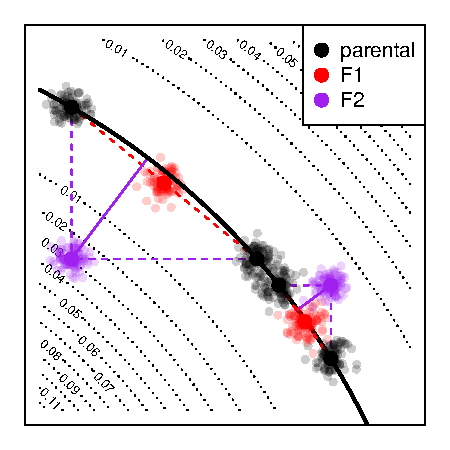
\includegraphics{figures/conceptual_fig}
\caption{
    \label{fig:conceptual_fig}
    A conceptual figure of the fitness consequences of hybridization:
    axes represent system coefficients (i.e., entries of $A$);
    the line of optimal system coefficients is down in black;
    dotted lines give phenotypic distances to the optimum.
    A pair of parental populations are shown in black, along the optimum;
    a hypothetical population of $F_1$s are shown in red,
    and the distribution of one type of $F_2$ is shown in purple
    (other types of $F_2$ are not shown; 
    some would be a similar distance to the other side of the optimal set).
    The distribution of $F_2$ hybrids is appropriate for mixed homozygotes
    if both traits have a simple, one-locus genetic basis,
    but there is variation within each population at that locus.
}
\end{figure}


\paragraph{Hybridization}
The means of two allopatric populations each of effective size $N_e$ separated for $T$ generations
will be a distance roughly of order $2\sigma_N \sqrt{T/N_e}$ apart along $\allS$. \revpoint{AE}{2}
(Consult figure \ref{fig:conceptual_fig} for a conceptual diagram.)
A population of $F_1$ hybrids has one haploid genome from each,
whose coefficients are averaged,
and so will have mean system coefficients at the midpoint between their means.
The distribution of $F_2$ hybrids will have mean at the average of the two populations,
but will have higher variance \citep{wright1968evolution,barton2001role,rosas2010cryptic}.
This ``segregation variance'' of $F_2$ hybrids 
can be shown to increase linearly with the square of the distance between
parental population means
under models of both simple and polygenic traits.
This is suggested by figure \ref{fig:conceptual_fig} and shown by \citet{slatkin1994segregation}
(also see Appendix \ref{apx:seg_cov} for a different derivation).
Concretely, we expect the population of $F_1$s to have variance $\sigma^2_S$ in the selected direction
(the same as within each parental population),
but the population of $F_2$ hybrids will have variance $\sigma^2_S + 4 \omega \sigma^2_N T/N_e$,
where $\omega$ is a factor that depends on the genetic basis of the coefficients.
If the optimal set $\allS$ has dimension $q$,
using the polygenic model of appendix \ref{apx:seg_cov}, 
$\omega$ is proportional to the number of degrees of freedom: $\omega = (p-q)/8$.
If each trait is controlled by a single locus, as in figure \ref{fig:conceptual_fig},
the value is similar.

%%% CITE SOME OF THESE
%% empirical data on sigma
% The amount and structure of this standing variation is established over long time scales
% by many factors, including mutation-selection balance, 
% shifts in the phenotypic optimum, and/or spatial variation in the optimum \citep{hansen1996translating}.
% Quantitative genetics models of mutation-selection balance 
% predict precise levels and structure of standing variation \citep{kimura_mutsel,lande_mutsel,lande1981models},
% but it is unclear how well these predictions match reality \citep{johnson_barton}
% and how much they are expected to change over time \citep{arnold_changing_G}.

What are the fitness consequences?
A population of $F_2$ hybrids will begin to be substantially less fit than the parentals
once they differ from the optimum by a distance of order $\gamma$,
i.e., once $\sqrt{4 \omega T/N_e} \approx \gamma / \sigma_N$.
This implies that hybrid incompatibility among $F_2$ hybrids should appear much slower --
on a time scale of $N_e (\gamma / \sigma_N)^2 / (4 \omega)$ generations.
The $F_1$s will not suffer fitness consequences until the hybrid mean is further than $\gamma$ from the optimum;
% as shown in appendix \ref{apx:away_from_opt} 
as suggested by figure \ref{fig:conceptual_fig}, Taylor expanding $D^2$ along the optimal set implies that
this deviation of the mean from optimum grows with the square of the distance between the parental populations,
and so we expect fitness costs in $F_1$s to appear on a time scale of $N_e^2$ generations.

% If a population has a Gaussian distribution of trait values with variance $\sigma^2$
% and fitness decays as $\exp(-x^2/2\gamma)$ away from the population mean,
% then the population mean fitness is 
% \begin{align*}
%    \int \frac{1}{\sigma \sqrt{2\pi}} e^{-\frac{x^2}{2\sigma^2}} e^{-\frac{x^2}{2\gamma^2}} dx
%    &=
%    \sqrt{\frac{1}{1 + (\sigma/\gamma)^2}}  \le \frac{1}{\sigma/\gamma} .
% \end{align*}
% If $\sigma$ is much smaller than $\gamma$, the fitness consequences of variation
% (i.e., genetic load) are small,
% but if $\sigma$ is of order $\gamma$, then mean fitness is inversely proportional to trait variance
% (i.e., $\gamma/\sigma$).
% This implies that we expect $\sigma_S < \gamma$
% but that once $T$ is of order $N_e (\gamma / \sigma_H)^2$, there will be loss of fitness
% in $F_2$ hybrids.
% Said another way,
% if we write $\mathcal{F}(T)$ as the mean fitness of an $F_2$ hybrid between two populations separated by $T$ generations,
% then fitness drops with the square root of $T$, measured in units of $N_e$ generations:
% \begin{align*}
%    \mathcal{F}(T) \le \frac{1}{\sigma_H/\gamma}\sqrt{\frac{N_e}{T}} .
% \end{align*}

For a more concrete prediction, suppose that the distribution among hybrids is Gaussian.
A population whose trait distribution is Gaussian with mean $\mu$ and variance $\sigma$,
has mean fitness 
\begin{align} \label{eqn:gauss_fit}
\int_{-\infty}^\infty \frac{1}{\sigma\sqrt{2\pi}} e^{-\frac{(x-\mu)^2}{2\sigma^2}} e^{-\frac{x^2}{2\gamma^2}} dx
&=
\sqrt{\frac{1}{1 + \sigma^2/\gamma^2}} \exp\left\{-\frac{\mu^2}{\gamma^2}\left(\frac{1}{1 + \sigma^2/\gamma^2}\right)\right\} .
% &\approx
% \frac{1}{\sigma/\gamma}\left(1 - \frac{\mu^2}{\gamma^2}\right) .
\end{align}
This assumes a single trait, for simplicity. %; the multivariate case is done in appendix \ref{apx:gauss_load}.
A population of $F_2$ hybrids will have, as above, variance $\sigma^2 = \sigma^2_S + 4 \omega \sigma^2_N T/N_e$.
The mean diverges with the square of the distance between the parentals, so we set $\mu = c_\mu \gamma T/N_e$,
where $c_\mu$ is a constant depending on the local geometry of the optimal set.
The mean fitness in parental populations is as in equation \ref{eqn:gauss_fit} with $\mu=0$ and $\sigma = \sigma_S$.
This implies that if we define $\fit_2(T)$ to be the mean relative fitness among $F_2$ hybrids
between two populations separated by $T$ generations, 
(i.e., the mean fitness divided by the mean fitness of the parents)
then
\begin{align} \label{eqn:fit2}
\fit_2(T) = 
  \left(1 + \frac{4 \omega (\sigma_N/\gamma)^2}{(1 + (\sigma_S/\gamma)^2)} \frac{T}{N_e} \right)^{-1/2} 
     \exp\left\{-\left(c_\mu \frac{T}{N_e}\right)^2 \left(\frac{1}{1 + (\sigma_S/\gamma)^2 + 4 \omega (\sigma_N/\gamma)^2 T/N_e}\right)\right\} .
\end{align}
If each of the $q$ selected directions acts independently,
the drop in fitness will be $\fit_2(T)^q$;
the expression for the correlated, multivariate case is given in Appendix \ref{apx:gauss_load}.
We discuss the implications of this expression in the next section.


%%%%%%%%%%
\paragraph{Speciation rates under neutrality}
Equation \eqref{eqn:fit2} describes how fast hybrids become inviable 
as the time that the parental populations are isolated increases;
what does this tell us about speciation rates under neutrality?
From equation \eqref{eqn:fit2} we observe that
time is always scaled in units of $N_e$ generations,
the population standard deviations are always scaled by $\gamma$,
and the most important term is the rate of accumulation of segregation variance,
$4 \omega (\sigma_N/\gamma)^2$.
All else being equal, this process will lead to speciation more quickly in smaller populations
and in populations with more neutral genetic variation (larger $\sigma_N$).
These parameters are related -- larger populations generally have more genetic variation --
but since these details depend on the situation, we leave these separate.

How does this prediction depend on the system size and constraint?
If there are $p$ trait dimensions, constrained in $q$ dimensions,
and if $\omega$ is proportional to $p-q$,
% the rate that hybrid variance increases with separation between parentals, $\omega$,
% is in some cases proportional to $p-q$, 
then the rate that $F_2$ fitness drops is, roughly,
$(1 + 4 (p-q) K T/N_e)^{-q/2} \propto q (p-q)$, where $K$ is a constant.
Both degree of constraint and number of available neutral directions
affect the speed of accumulation of incompatibilities --
more unconstrained directions allows faster system drift,
but more constrained directions implies greater fitness consequences of hybridization.
However, note that in real systems, it is likely that $\gamma$ also depends on $p$ and $q$.

Now we will interpret equation \eqref{eqn:fit2} in three situations plausible for different species,
depicting how hybrid fitness drops as a function of $T/N_e$ in Figure \ref{fig:speciation_rates}.
In all cases, the fitness drop for $F_1$ hybrids is much smaller than that of $F_2$ hybrids,
so we work only with the first (square-root) term in equation \eqref{eqn:fit2}.

% simgaN = sigmaS = gamma, large population
Suppose in a large, genetically diverse population,
the amount of heritable variation in the neutral and selected directions are roughly equal 
($\sigma_N \approx \sigma_S$)
but the overall amount of variation is (weakly) constrained by selection
($\sigma_N \approx \gamma$).
If so, then the first term of equation \eqref{eqn:fit2} is
$1/\sqrt{1 + 2 \omega T/N_e} \approx 1 - \omega T/N_e$.
If also $\omega=1$, then, for instance, after $0.1 N_e$ generations
the average $F_2$ fitness has dropped by 10\% relative to the parentals.

%  $\sigma_N \approx \sigma_S \ll \gamma$, ``isolated population''
Consider instead a much smaller, isolated population
whose genetic variation is primarily constrained by genetic drift,
so that $\sigma_N \approx \sigma_S \ll \gamma$.
Setting $a = (\sigma_N/\gamma)^2$ to be small,
the fitness of $F_2$ hybrids is $\fit_2 \le 1/\sqrt{1 + 4 \omega a T/N_e} \approx 1 - 2 \omega a T/N_e$.
Hybrid fitness seems to drop more slowly in this case in figure \ref{fig:speciation_rates},
but since time is scaled by $N_e$, so speciation may occur \emph{faster} than in a large population.
However, at least in some models \citep{lynch1986phenotypic}, in small populations at mutation-drift equilibrium
the amount of genetic variance ($\sigma_N^2$) is proportional to $N_e$,
which would compensate for this difference, 
perhaps even predicting the rate of decrease of hybrid fitness to be independent of population size
for small populations.

% $\sigma_N \gg \sigma_S \approx \gamma$, if $N_e$ is big and there's a lot of recombination load (``species complex'')
In the other direction, consider large metapopulations (or a ``species complex'')
among which heritable variation is strongly constrained by selection
(i.e., there is substantial recombination load),
so that $\sigma_S \approx \gamma$ but $\sigma_N/\gamma$ is large.
Then the fitness of $F_2$ hybrids is $\fit_2 \le 1/\sqrt{1 + 2 \omega a T/N_e} \approx 1 - \omega a T/N_e$,
and could be extremely rapid if $a$ is large.

For instance, between two populations of one million organisms that has 10 generations per year (a drosophilid species, perhaps)
under the ``large population'' scenario of Figure \ref{fig:speciation_rates}A,
system drift would lead to a substantial fitness drop of around 10\% in $F_2$ hybrids in only 10,000 years.
This drop may be enough to induce evolutionary reinforcement of reproductive isolation.
If one thousand of these organisms is isolated (perhaps on an island, as in Figure~\ref{fig:speciation_rates}B),
then a similar drop could occur in around 120 years.
On the other hand, if the population is one of several of similar size
that have recently come into secondary contact after population re-expansion,
the situation may be similar to that of Figure~\ref{fig:speciation_rates}C with $N_e = 10^6$,
and so the same drop could occur after 1,100 years.
(However, hyperdiverse populations of this last type may not be stable on these time scales.)


\begin{figure}[H]
\begin{center}
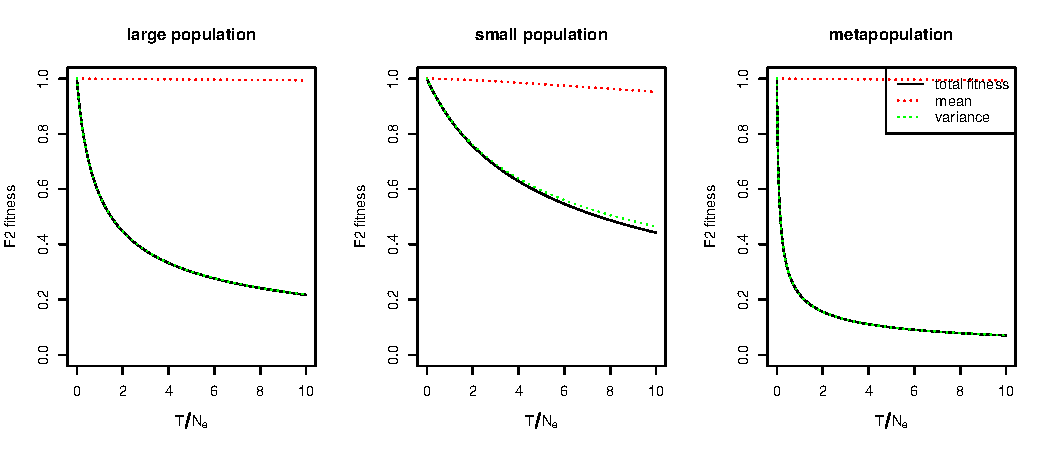
\includegraphics{speciation_rates}
\caption{
Mean drop of $F_1$ and $F_2$ fitness relative to parental species,
with $\omega=1$ and 
\textbf{(A)} $\sigma_N^2 = \sigma_S^2 = \gamma^2$
\textbf{(B)} $\sigma_N^2 = \sigma_S^2 = 0.1 \gamma^2$
\textbf{(C)} $0.1 \sigma_N^2 = \sigma_S^2 = \gamma^2$.
The $F_2$ fitness is from equation \eqref{eqn:fit2},
and the $F_1$ fitness is determined only by the exponential term of that equation,
which is small relative to that of increased variance.
\label{fig:speciation_rates}}
\end{center}
\end{figure}


%%%%%%%%%%%%%%%%%%%%%%%%
\section*{Discussion}

This simple quantitative genetics model we use above
has been shown to produce good predictions in many situations,
even when the substantial number of simplifying assumptions are violated \citep{burger1994distribution,turelli1994genetic}.
The calculations above should be fairly robust even to substantial deviations from normality.
A larger effect on these predictions seems likely due to 
correlations due to molecular constraint, genetic linkage, population structure, historical contingency and so forth.
Although such considerations would not change the qualitative predictions of this model,
their combined effects could substantially change the predicted rate of accumulation of incompatibilities.

%% Fisher's geometric model
% Differences:
% - they look at shifting environments too
% - they just model substitutions, so only hybrids have genetic variance
% chevin2014niche:
% - m is accessible, constrained dimensionlity (allows for a ridge)
% - predicts rate of RI accumulation (due to substitutions) is \propto N^{-(1+m/2)}
%   since this is mean log fitnees; says hybrids will have fitness
%     exp( - m C T N^{-(1+m/2)} ) ~ 1 - m C T N^(-(1+m/2))
% - says RI accum is *faster* at higher m but this is not obv frm eqns
% - we say it should be ( exp(-C (T/N)^2) / sqrt(T/N) )^m :
%     ~ 1 - m C (T/N)

\paragraph{Fisher's geometric model}
Substantial analytical work on speciation has been done using Fisher's geometric model, 
which can also predict Haldane's rule and the regular increase of incompatibility with genetic distance
\citep{barton2001role,fraisse2016genetics,simon2017coadapted}.
The model is similar to the quantitative genetics model we use 
to predict the rate of speciation, 
although work on Fisher's geometric model generally only models substitutions
between populations, neglecting within-species polymorphism.
Indeed, our model may provide an additional mechanistic context 
in which Fisher's geometric model is appropriate,
although the typical degree of pleiotropy
and stability of the $G$-matrix are unknown in practice.
Our observations argue that for questions related to divergence between populations 
it may be important to model a non-point optimum,
as is in \citet{chevin2014niche}. \revpoint{AE}{3}

Although our main focus is on the implications of system theory,
rather than on the quantitative genetics modeling,
it is interesting to compare analytic results.
\citet{chevin2014niche} finds that mean fitness decrease of hybrids
after $T$ generations grows proportionally to $m N_e^{-1-m/2} T$, for large $N_e$;
while our corresponding rate is $m T / N_e$.
This difference in time scaling is substantial, especially for large populations,
and seems to appear because \citet{chevin2014niche} uses the results of \citet{sella2005application}
to describe how the steady-state fitness and substitution process
depends on trait dimensionality
(the fitness peak is harder to find in higher dimensions).
We do not incorporate this effect
because genetic variation may be provided by other sources,
but if we did, it would enter through our $\sigma_S$.

\section*{Acknowledgements}

    We would like to thank Sergey Nuzhdin, Stevan Arnold, Michael Turelli, Patrick Phillips, Erik Lundgren and Hossein Asgharian for valuable discussion. 
    We would also like to thank Nick Barton, Sarah Signor, Todd Parsons, Joachim Hermisson for very helpful comments on the manuscript.
    Work on this project was supported by funds from
    the Sloan Foundation and the NSF (under DBI-1262645) to PR.



\bibliographystyle{plainnat}
\bibliography{krefs}
%\end{multicols}

\normalsize
\appendix


%%%%%%%%%%%%%%%%%%%%%%%%%%%%%%%%%%%%%%%%%%%%%%%%
\section{Genetic drift with a multivariate trait}
\label{ss:quant_gen}

For completeness, we provide a brief exposition of how a population 
evolves due to genetic drift
with a quantitative genetics model,
as in \citet{lande1981models} or \citet{hansen1996translating}.
These do not directly model underlying genetic basis,
but developing a more accurate model is beyond the scope of this paper.

Suppose that the population is distributed in trait space
as a Gaussian with covariance matrix $\Sigma$ and mean $\mu$,
whose density we write as $f(\cdot;\Sigma,\mu)$.
Selection has the effect of multiplying this density by the fitness function and renormalizing,
so that if expected fitness of $x$ is proportional to $\exp(-\|Lx\|^2/2)$,
then the distribution post-selection
has density at $x$ proportional to $f(x;\Sigma,\mu) \exp(-\|Lx\|^2/2)$.
By the computation below (``Completing the square''),
the result is a Gaussian distribution
with covariance matrix $(\Sigma^{-1} + L^T L)^{-1}$ 
and mean $(\Sigma^{-1}+L^T L)^{-1} \Sigma^{-1} \mu$.
% Importantly, if $U$ is not invertible, then by $U^{-1}$ 
% we mean $(U^T U)^{-1} U^T$, Moore-Penrose pseudoinverse of $U$,
% so that $U U^{-1}$ is equal to the projection matrix
% onto the span of the columns of $U$.

After selection, we have reproduction:
suppose this occurs as in the infinitesimal model \citep{barton2017infinitesimal},
so that each offspring of parents with traits $x$ and $y$
is drawn independently from a Gaussian distribution 
with mean $(x+y)/2$ and covariance matrix $R$.
Here, $R$ is the contribution of ``segregation variance'',
i.e., random choices of parental alleles.
If $\widetilde \Sigma = (\Sigma^{-1} + L^T L)^{-1}$ 
is the covariance matrix of the parents post-selection,
then the distribution of offspring will again be Gaussian,
with mean equal to that of the parents
and covariance matrix $\widetilde \Sigma/2 + R$.

In summary, a generation under this model modifies the mean ($\mu$)
and covariance matrix ($\Sigma$) of a population as follows:
\begin{align*}
    \mu &\mapsto \mu' = (\Sigma^{-1}+L^T L)^{-1} \Sigma^{-1} \mu \\
    \Sigma &\mapsto \Sigma' = \frac{1}{2} (\Sigma^{-1} + L^T L)^{-1} + R .
\end{align*}
What measures are stable under this transformation?
The condition $\mu = \mu'$ reduces to $\Sigma L^T L \mu = 0$;
if we assume $R$ and therefore $\Sigma$ are of full rank,
then this happens if and only if $\mu$ is in the null space of $L$,
i.e., if $\mu$ lies in a neutral direction.
The condition $\Sigma' = \Sigma$ can also be solved,
at least numerically.
After rearrangement, it reduces to
$\Sigma L^T L \Sigma + (I/2 - R L^T L) \Sigma = R$.
%% I DON'T THINK WE USE THE FOLLOWING:
% We can find a more explicit description
% if we assume that $x^T L^T L x = \sum_{i=1}^k x_i^2$,
% i.e., that selection only cares about the first $k$ coordinates,
% and then with no interactions between traits.
% If so, the condition $\Sigma' = \Sigma$
% can be written in block form as
% \begin{align*}
%     \begin{bmatrix}
%         \Sigma_{11}^2 + (I/2 - R_{11}) \Sigma_{11}
%         & \Sigma_{11} \Sigma_{12} + (I/2 - R_{11})\Sigma_{12} \\
%         \Sigma_{12}^T \Sigma_{11} + \Sigma_{12}^T/2 - R_{12}^T \Sigma_{11}
%         & \Sigma_{22} - R_{12}^T \Sigma_{12} 
%     \end{bmatrix}
%     &=
%     \begin{bmatrix}
%         R_{11} & R_{12} \\
%         R_{12}^T & R_{22}
%     \end{bmatrix} .
% \end{align*}
% The first equation, $\Sigma_{11}^2 + (I/2 - R_{11}) \Sigma_{11} = R_{11}$,
% can be solved with the quadratic formula: 
% $$\Sigma_{11} = (R_{11} - I/2 + Q)/2$$
% for any $Q$ that commutes with $R_{11}$
% and is a solution to $Q^2 = (R_{11} - I/2)^2 + 4 R_{11}$.
% Since we need $\Sigma$ to be positive definite,
% we take the solution with positive eigenvalues.
% Given $\Sigma_{11}$, the remaining components are
% \begin{align*}
%     \Sigma_{12} 
%     &= 
%     \left( \Sigma_{11} + I/2 - R_{11} \right)^{-1} R_{12} \\
%     \Sigma_{22}
%     &=
%     R_{12}^T \Sigma_{12} + R_{22} .
% \end{align*}
Importantly, the mean $\mu$ does not affect 
either how the covariance matrix moves,
or its stable shape.

Above we have described the \emph{expected} motion of the mean and covariance.
However, random resampling will introduce noise.
Suppose that a population of $N$ individuals
behaves approximately as described above.
By the above,
we may expect that the covariance matrix stays close to a constant value $\Sigma$,
computed from $R$ and $L$ as above,
so that we need only consider motion of the mean, $\mu$.
Since we take a sample of size $N$ to construct the next generation,
the next generation's mean is drawn from a Gaussian distribution with mean $\mu'$
and covariance matrix $\Sigma/N$.
Defining $\Gamma = (I - (I + \Sigma L^T L)^{-1})$,
this can be written as
\begin{align*}
    \mu' - \mu = \Gamma \mu + \epsilon/\sqrt{N} ,
\end{align*}
where $\epsilon$ is a multivariate Gaussian with mean zero and covariance matrix $\Sigma$.
Let $\mu(k)$ denote the mean in the $k^\text{th}$ generation,
and suppose that $\mu$ differs from optimal by something of order $1/\sqrt{N}$:
if $\nu(t) = \sqrt{N} \mu(t\sqrt{N})$ is the rescaled process,
then the previous equation implies that as $N \to \infty$, 
in the limit $\nu$ solves the It\^{o} equation
\begin{align*}
    d \nu(t) = \Gamma \nu(t) dt + \Sigma^{1/2} dW(t) ,
\end{align*}
where now $W(t)$ is a multivariate white noise.
This has an explicit solution as a multivariate Ornstein-Uhlenbeck process:
\begin{align*}
    \nu(t) = e^{-t \Gamma} \nu(0) + \int_0^t e^{-(t-s) \Gamma} \Sigma^{1/2} dW(s).
\end{align*}
% Note that after some algebra, $\Gamma = \Sigma L^T L (I - \Sigma L^T L)^{-1}$.
The asymptotic variance of this process in the direction $z$ is
\begin{align} \label{eqn:limiting_cov}
    \lim_{t \to \infty} \var[\nu(t) \cdot z]
    &=
    \int_0^\infty z^T e^{-s \Gamma} \Sigma e^{-s \Gamma} z ds ,
\end{align}
which is infinite if and only if $\Gamma z = 0$,
which occurs if and only if $Lz=0$.
This implies that at equilibrium, 
population mean trait values lie away from the optimal set
by a Gaussian displacement of order $1/\sqrt{N}$
with a covariance matrix given by equation \eqref{eqn:limiting_cov}.


\paragraph{Completing the square}
First note that if $A$ is symmetric,
\begin{align*}
    (x-y)^T A (x-y)
    &=
    x^T A \left( x - 2y \right) + y^T A y ,
\end{align*}
and so if $B$ is also symmetric and $A+B$ is invertible,
\begin{align*}
    (x-y)^T A (x-y) + x^T B x
    &=
    x^T (A + B) \left( x - 2 (A + B)^{-1} A y \right) + y^T A y \\
    &=
    \left( x - (A + B)^{-1} A y \right)^T
    (A + B)
    \left( x - (A + B)^{-1} A y \right) \\
    &\qquad{}
    + y^T A y - y^T A^T (A+B)^{-1} A y .
\end{align*}
Therefore, 
by substituting $A=\Sigma^{-1}$ and $B=L^T L$,
\begin{align*}
    \frac{ f(x;\Sigma,y) \exp(-x^T L^T L x / 2)}{\int f(z;\Sigma,y) \exp(-z^T L^T L z / 2) dz}
    &=
    f(x; (\Sigma^{-1} + L^T L)^{-1}, (\Sigma^{-1}+L^T L)^{-1} \Sigma^{-1} y) .
\end{align*}

%%%%%%%%%%%%%%%%%%%%%%%%%%%%%%%
\subsection{Gaussian load}
\label{apx:gauss_load}

Suppose that a population has a Gaussian distribution in $d$-dimensional trait space
with mean $\mu$ and covariance matrix $\Sigma$,
and that fitness of an individual at $x$ is $\exp(-\|Lx\|^2/2)$.
Then, completing the square as above with $A=\Sigma^{-1}$, $y=\mu$, and $B=L^T L$,
and defining $Q = (\Sigma^{-1} + L^T L)^{-1}$,
\begin{align*}
    &
    \frac{1}{\sqrt{2 \pi}^n \det(\Sigma)^{1/2}} 
        \int e^{-\frac{1}{2} x^T \Sigma^{-1} x} e^{-\frac{1}{2} x^T L^T L x} dx \\
    &\qquad =
    \frac{1}{\sqrt{2 \pi}^n \det(\Sigma)^{1/2}} 
        \int e^{-\frac{1}{2}(x-Q \Sigma^{-1} \mu)^T Q^{-1} (x-Q \Sigma^{-1} \mu)} dx 
        \\ &\qquad \qquad {}
        \times e^{\mu^T \left( I - \Sigma^{-1} Q \right) \Sigma^{-1} \mu} \\
    &\qquad =
    \sqrt{\frac{\det(Q)}{\det(\Sigma)}}
        \exp\left\{\mu^T \left( I - \Sigma^{-1} Q \right) \Sigma^{-1} \mu\right\} \\
    &\qquad =
    \sqrt{\frac{1}{\det(\Sigma)\det(\Sigma^{-1}+L^TL)}}
        \exp\left\{\mu^T \left( I - (I + L^T L \Sigma)^{-1} \right) \Sigma^{-1} \mu\right\} \\
\end{align*}
This is the product of two terms:
the first gives the drop in fitness due to segregation variance,
and the second the drop due to a shift in mean away from the optimum.
A similar decomposition appears in \citet{barton2001role} and \citet{chevin2014niche},
but for mean log fitness.

Now suppose that $\Sigma = \sigma^2 I$ and $L = I/\gamma$.
Then,
\begin{align*}
    \sqrt{\frac{1}{\det(\Sigma)\det(\Sigma^{-1}+L^TL)}}
    &=
    \sqrt{\frac{1}{\sigma^{2d} (1/\sigma^2 + 1/\gamma^2)^d}} \\
    &=
    \frac{1}{(1+ \left(\sigma/\gamma\right)^2)^{d/2}} .
\end{align*}
Also, 
\begin{align*}
        \left( I - (I + L^T L \Sigma)^{-1} \right) \Sigma^{-1} 
        &=
        \frac{1}{\sigma^2}\left( 1 - (1 + (\sigma/\gamma)^2)^{-1} \right) I \\
        &=
        \frac{1}{\gamma^2}\frac{1}{(1 + (\sigma/\gamma)^2)} I \\
\end{align*}


%%%%%%%%%%%
\section{Evolution of segregation covariance}
\label{apx:seg_cov}

The description above does not describe how \emph{two} diverging populations interact,
since the amount of \emph{segregation variance}, quantified by $R$,
will not stay constant.
This has been quantified in various models before
\citep[e.g.,][]{slatkin1994segregation,barton2001role,chevin2014niche};
we provide the following calculations for completeness.

To get an idea of how segregation variance might evolve,
suppose that a trait is determined by $L$ unlinked, biallelic loci,
and that the $i^\mathrm{th}$ locus has two alleles with additive effects $\pm \alpha_i$,
so that being homozygous for the $+$ allele contributes $+2 \alpha_i$ to the trait.
For simplicity, we will neglect the effects of selection.
If the $+$ allele at locus $i$ is at frequency $p_i$ in a population,
then the mean and genetic variance of the trait in a diploid population with random mating is
\begin{align*}
    m &= 2 \sum_i (2 p_i - 1) \alpha_i \\
    s^2 &= 4 \sum_i p_i (1-p_i) \alpha_i^2 .
\end{align*}


Segregation variance between two parents depends on the loci at which either are heterozygous,
and each locus contributes independently
since alleles are additive.
If the alleles are at Hardy-Weinberg proportions,
then since segregation acts like a fair coin flip, a heterozygous locus contributes $\alpha_i^2/4$ to the variance,
and so the \emph{mean} segregation variance, averaging across parents, is
% two parents, prob 2p(1-p) for prob the locus is heterozygous, variance 0.5(1-0.5)\alpha^2.
\begin{align*}
    R_0(p) = \sum_i p_i (1-p_i) \alpha_i^2 .
\end{align*}

On the other hand,
if the second parent came from a distinct population
with frequencies $q_i$
(an $F_1$ hybrid),
this would be
\begin{align*}
    R_1(p,q) &= \frac{1}{2} \sum_i p_i^2 (1-p_i)^2 \alpha_i^2 
                + \frac{1}{2} \sum_i q_i^2 (1-q_i)^2 \alpha_i^2 \\
                &= (R_0(p) + R_0(q))/2 .
\end{align*}
If we assume that the populations are at equilibrium, $R_0(p) \approx R_0(q)$,
and so $R_1(p,q) \approx R_0(p)$.

Now consider an $F_2$ hybrid, where both parents are $F_1$
and so each heterozygous at locus $i$ with probability $p_i (1-q_i) + (1-p_i) q_i$.
Then
\begin{align*}
    R_2(p,q) &= \frac{1}{2} \sum_i \left(p_i (1-q_i) + (1-p_i) q_i \right) \alpha_i^2  .
\end{align*}
Suppose that the two populations are slightly drifted from each other,
with frequency difference $p_i-q_i = 2\epsilon_i$.
Then,
\begin{align*}
    p (1-q) + p (1-q)
    &=
    (u+\epsilon) (1-u+\epsilon) + (u-\epsilon) (1-u-\epsilon) \\
    &=
    2 u (1-u)
    % + \epsilon (u + (1-u) - u - (1-u))
    + 2 \epsilon^2 .
\end{align*}
If the frequencies have evolved neutrally in unconnected, Wright-Fisher populations 
of effective size $N$ for $t$ generations from a common ancestor with allele frequency $u$,
then $\epsilon$ has mean zero and variance roughly $2 u (1-u) t/N$.
Still assuming the populations are at stationarity,
so that $R_0$ is constant between the two,
and taking the frequencies $p_i$ as a proxy for the ancestral frequencies $u_i$,
this implies that we expect
\begin{align*}
    R_2 
    &\approx 
    R_0 + 2 \sum_i p_i (1-p_i) \alpha_i^2 t/N \\
    &=
    \left( 1 + \frac{2t}{N} \right) R_0 .
\end{align*}
On the other hand, the expected squared difference in trait \emph{means} between two such populations is
\begin{align} \label{eqn:var_dx}
    8 \sum_i p_i (1-p_i) \alpha_i^2 t / N = 8 R_0 t /N .
\end{align}
This implies that under this model,
segregation variance in $F_2$ hybrids between two populations
is roughly increased by a factor of $1/8$ of the difference between their means.


% reviews here if toggled above
% \ifsubmission\processdelayedfloats\fi

\includereviews


\end{document}
